\documentclass[main]{subfiles}


\begin{document}
\newpage
\section{Neuromorphic Systems 2} \label{l12}

\subsection{Neuromorphic approaches}
Neuromorphic Engineering has its roots in the in the early 70' \textit{subterranean group}, formed by Carver Mead, Max Delbruck and Paul Mueller. This group studied membrane channel biophysics showing the all-or-nothing property of single channels and that membrane conductance was a function of the fractional population of channels in the open state. The group also developed methods based on statistics of current flow that enabled them to measure single channel current and the shape of the energy barrier.

After the group ended it's work, Carver turned his whole lab to the pursuit of neuromorphic electronic engineering while working on the first silicon retina chip with Misha Mahovald, an undergraduate biology student. They published it in 1991.
Also in 1991, Misha Mahovald and Rodney Douglas proposed a conductance-based silicon neuron and showed that it had properties remarkably similar to those of real cortical neurons.

Neuromorphic computing is today present in many digital and mixed-signal devices, encompassing a wide-range of approaches. Some of examples are:
\begin{enumerate}
    \item ARM-based simulated spiking neural networks: SpiNNaKer - a custom digital computing architecture that is fully programmable, provides fixed-point arithmetic in pseudo real-time and is optimized for spiking computational neuroscience simulations
    \item Asynchronous simulation of neurons and synapses: Loihi - an asynchronous multi-core chip for simulating spiking neural networks and on-chip learning. It has a low-power consumption and is optimised for prototyping and scalability.
    \item Large-scale asynchronous spiking neural network: TrueNorth - an asynchronous multi-core, large-scale spiking neural network fabric. It is reconfigurable, has binary (1 bit) synapses and computes everything in pseudo real-time with 1 ms frames. It is optimized for low-power and low-latency processing tasks.
    \item Wafer-scale analog neural accelerators: BrainScaleS - a full custom large-scale analog-digital neural processing system. It has limited precision due to it's analog components but works in accelerated time (x1000) and is designed for faithful reproduction of neuroscience simulations.
    \item Real-time neuromorphic large-scale system: BrainDrop - a full custom analog-digital neural engineering framework computing engine. It works in analog subthreshold so it is noisy and has limited precision. It is a real-time system with ultra-low power-consumption that is scalable but has no on-chip learning.
    \item Real-time on-line learning neuromorphic chips: DYNAPs - a full custom analog-digital models of cortical circuits. Uses analog subthreshold and thus is noisy and has limited precision but provides real-time and ultra-low power computation. It is scalable and onlie reconfigurable. It is desinged for implementing principles of neural computatoin in real-time behaving agents.
\end{enumerate}

Thus all the efforts put into this field can be divided in three large directions:

\begin{enumerate}
    \item Neuromorphic Engineering - represents the fundamental research done in this field on emulating neural function using subthreshold analog circuits and asynchronous digital chips.
    \item Neuromorphic Computing - is application driven and can be seen as a conservative approach including simulating neural networks and building custom VLSI circuits.
    \item Neuromorphic Devices - is oriented towards new emerging memory technologies like memristive devices, the use of in-memory computing and high-density arrays.
\end{enumerate}{}

\subsection{Neuromorphic electronic circuits}

\subsubsection{The approach}
The neuromorphic engineering approach is centered on learning to build artificial neural processing systems that can interact intelligently with the physical world. It combines multiple disciplines such as neuroscience physics, computer science, electrical engineering etc. It exploits device physics to directly emulate biophysical properties of neural systems. Biophysical processes happen in time so in this approach time is represented implicitly in the physical processes the produce emulating computation, without explicit time references in these circuits. This approach aims to implement robust computation in autonomous egents leading to cognitive behavior.

Why analog subthreshold? See the first part of the previous lecture.

Neuromorphic computation has represented a radical paradigm shift by challenging well-established assumptions poised by conventional computing architectures (e.g. von Neumann). 

The first essential property of neuromorphic computing is this ability to exploit physical space more efficiently through fine grain parallelism, not needing time-multiplexing of multiple tasks onto common resources. Memory and computation are co-localized reducing data transfer time and storage problems. Neurons generally don't activate all at the same time (excepting in case of conditions like Epilepsy), thus they can be though of as sparsely activating in space and time, as opposed to conventional computers which can use most of their computing resources at a point in time. Neuromorphic circuits can be driven only at the arrival of an input signal, thus they can inherently exploit the data-driven computational paradigm.

The second property is that time is represented implicitly allowing for real-time interaction with the environment. By modulating circuit time constants, one can adjust responses with input signal dynamics. This property allows neuromorphic circuits to be synchronized with real-world events by default while providing low-power and low-bandwidth processing of sensory signals.

\subsubsection{Analog circuits}

Current-mode CMOS circuits operated in the subthreshold, or weak-inversion, regime can be used to implement log-domain filters. Current-mode log-domain CMOS filters have favorable properties, such as wide dynamic range at low supply voltage, compactness, linearity and low power consumption. These properties are becoming increasingly important for biomedical applications that require extremely low-power dissipation and neuromorphic circuits that attempt to reproduce the biophysics of biological neurons and synapses. [cite giacomo & ..]

An example of classical log-domain integrator is presented in Figure \ref{fig:log-dom}. This circuit’s linear transfer function can be easily derived by applying the translinear principle on the $V_{gs}$ loop highlighted by the arrows: given the exponential relationship between the subthreshold currents of the p-FETs and their $V_{gs}$ voltages we can write: $I_{th} \cdot I_1 = I_2 \cdot I_{out}$. In subthreshold, the output n-FET $M_{out}$ produces a current that changes exponentially with its gate voltage $V_c$. Differentiating $I_out$ with respect to $V_c$ and combining the result with the capacitor equation $C\frac{d}{dt}V_{C} = I_{2}-I_{\tau}$ we obtain:

\begin{equation}
    \tau \frac{d}{dt}I_{out} + I_{out} = \frac{I_{th}}{I_{\tau}} I_{in}
\end{equation}{}

\begin{figure}[h]
    \centering
    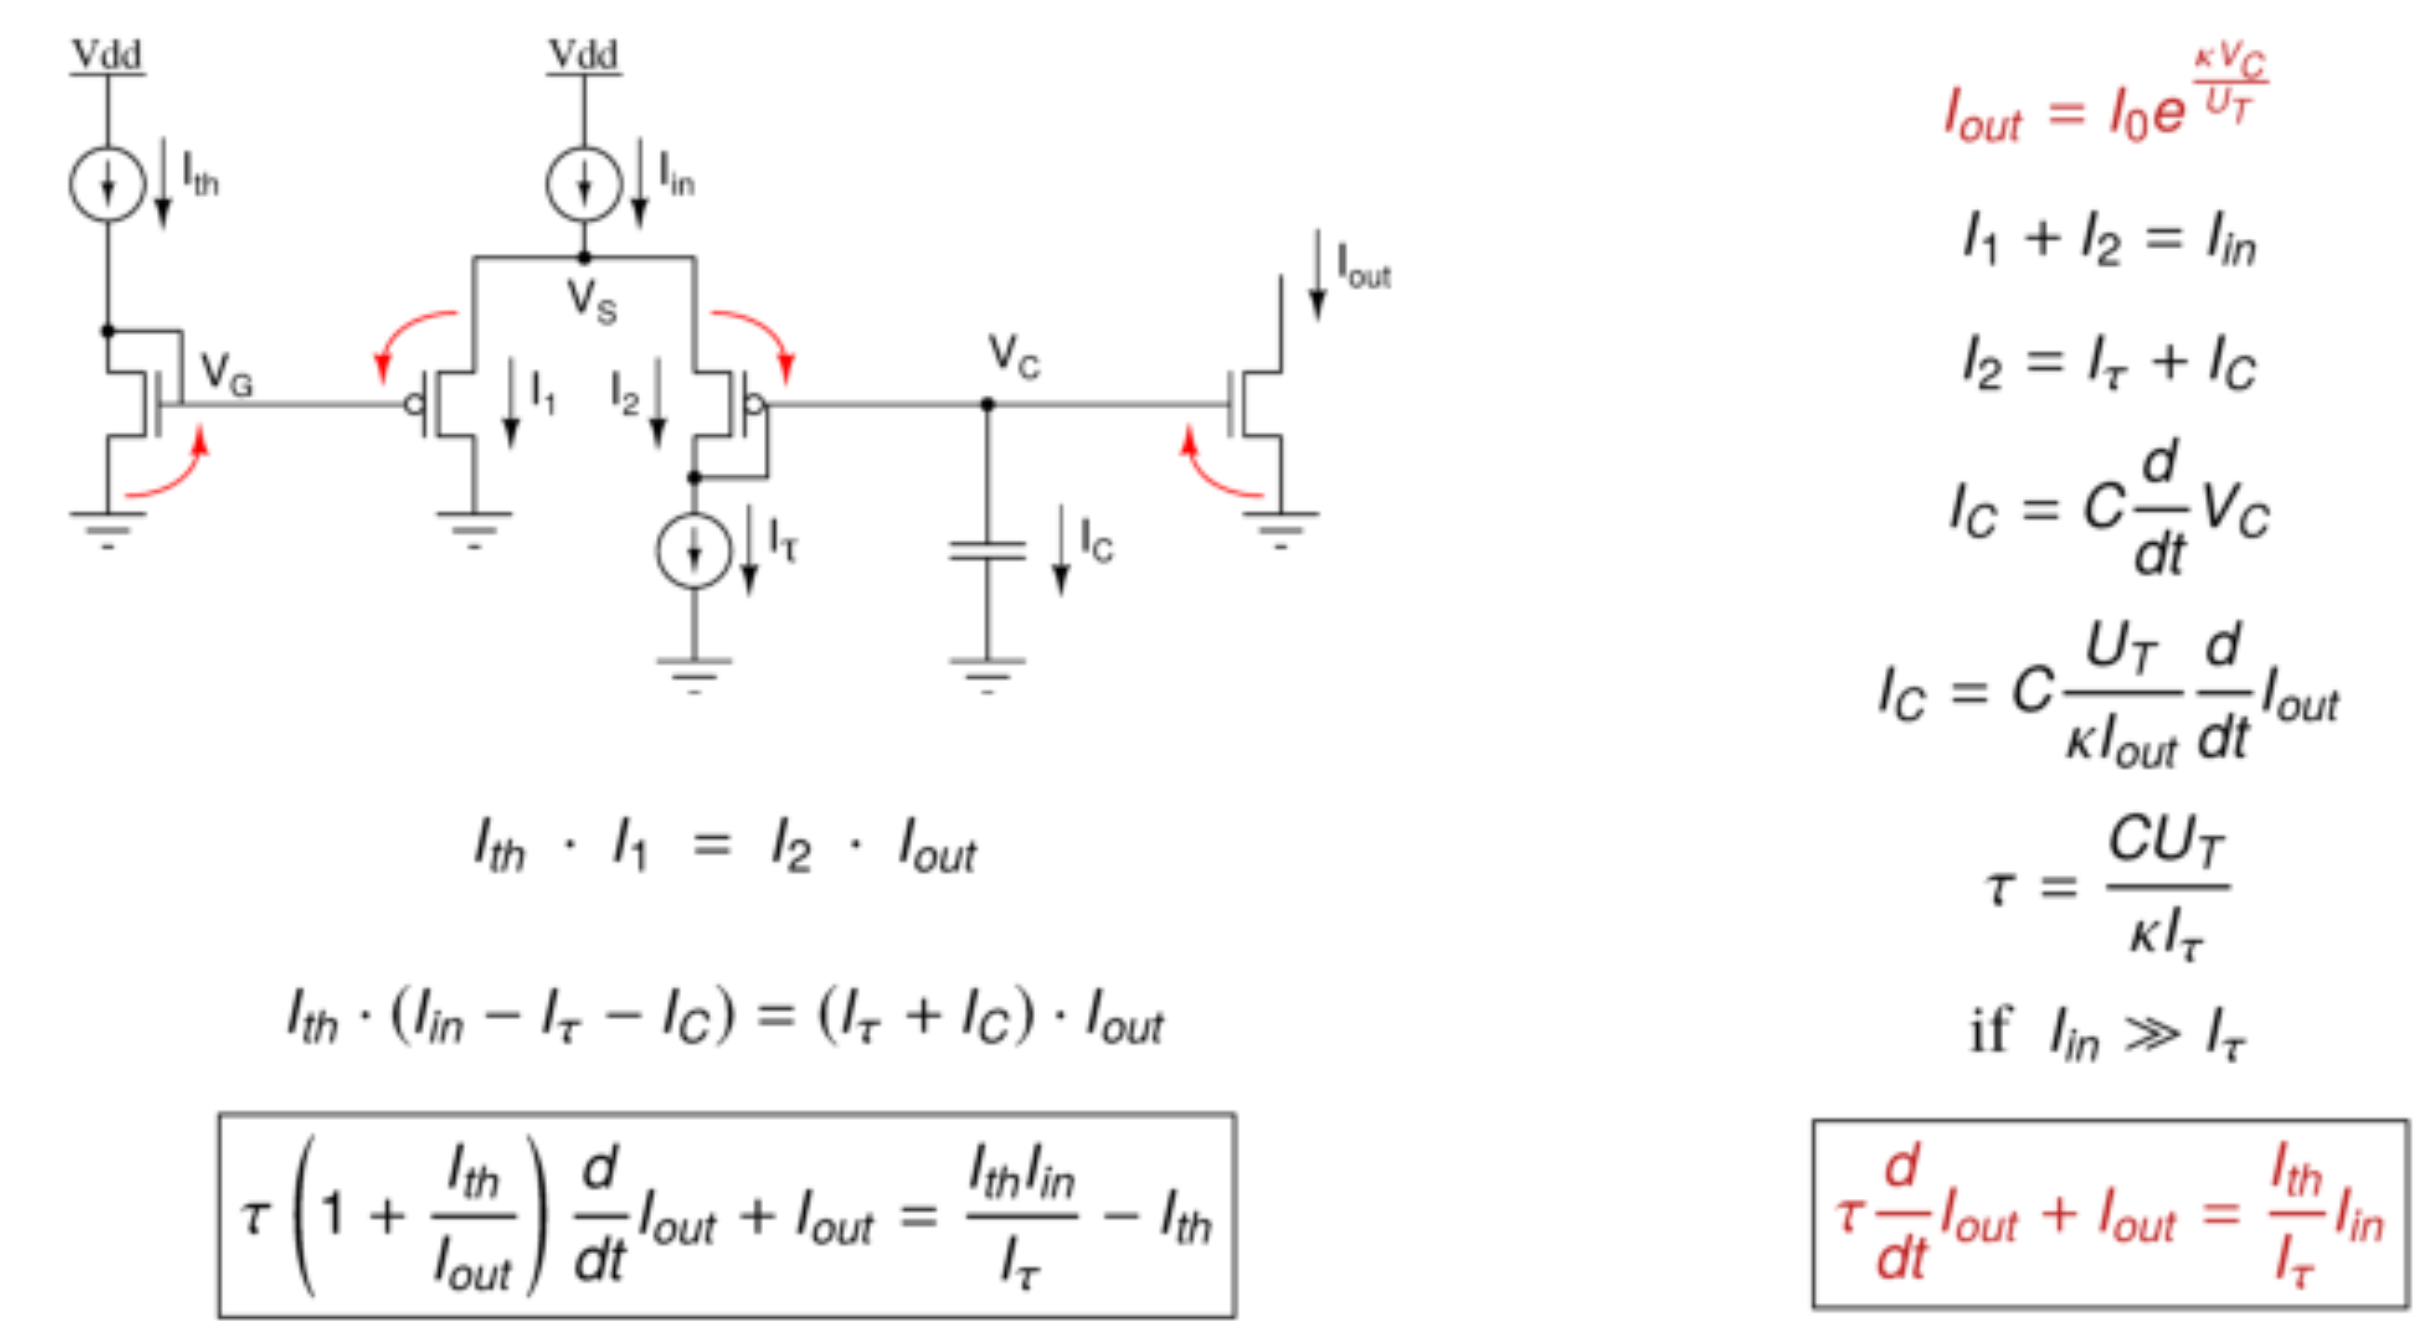
\includegraphics[width=0.8\linewidth]{12_NeuromorphicSystems2/figures/log-dom.PNG}
    \caption{Classical log-domain integrator.}
    \label{fig:log-dom}
\end{figure}
%

The DPI is a CMOS current-mode circuit that operates in the subthreshold regime integrating voltage pulses. However, rather than using a single pFET to generate the appropriate $I_w$ current, via the translinear principle (Gilbert, 1975), it uses a differential pair in negative feedback configuration. This allows the circuit to achieve LPF functionality with tunable dynamic conductances: Input voltage pulses are integrated to produce an output current that has maximum amplitude set by $V_w$, $V_t$, and $V_{thr}$. [silicon neuron circuits] It has additional advantages of providing a compact layout, better matching properties and lower power consumption. The \textbf{differential-pair integrator} is used to model synaptic dynamics.

It comprises only 3 n-FETs, 2 p-FETs and 1 capacitor. The two current sources are implemented using two subthreshold MOSFETs: one n-FET for the $I_{in}$ current and one p-FET for the $I_t$ current. Following a similar derivation to the one used in the classical log-domain integrator, the characteristic equation is obtained as observed in Figure \ref{fig:dpi}

%
\begin{figure}[h]
    \centering
    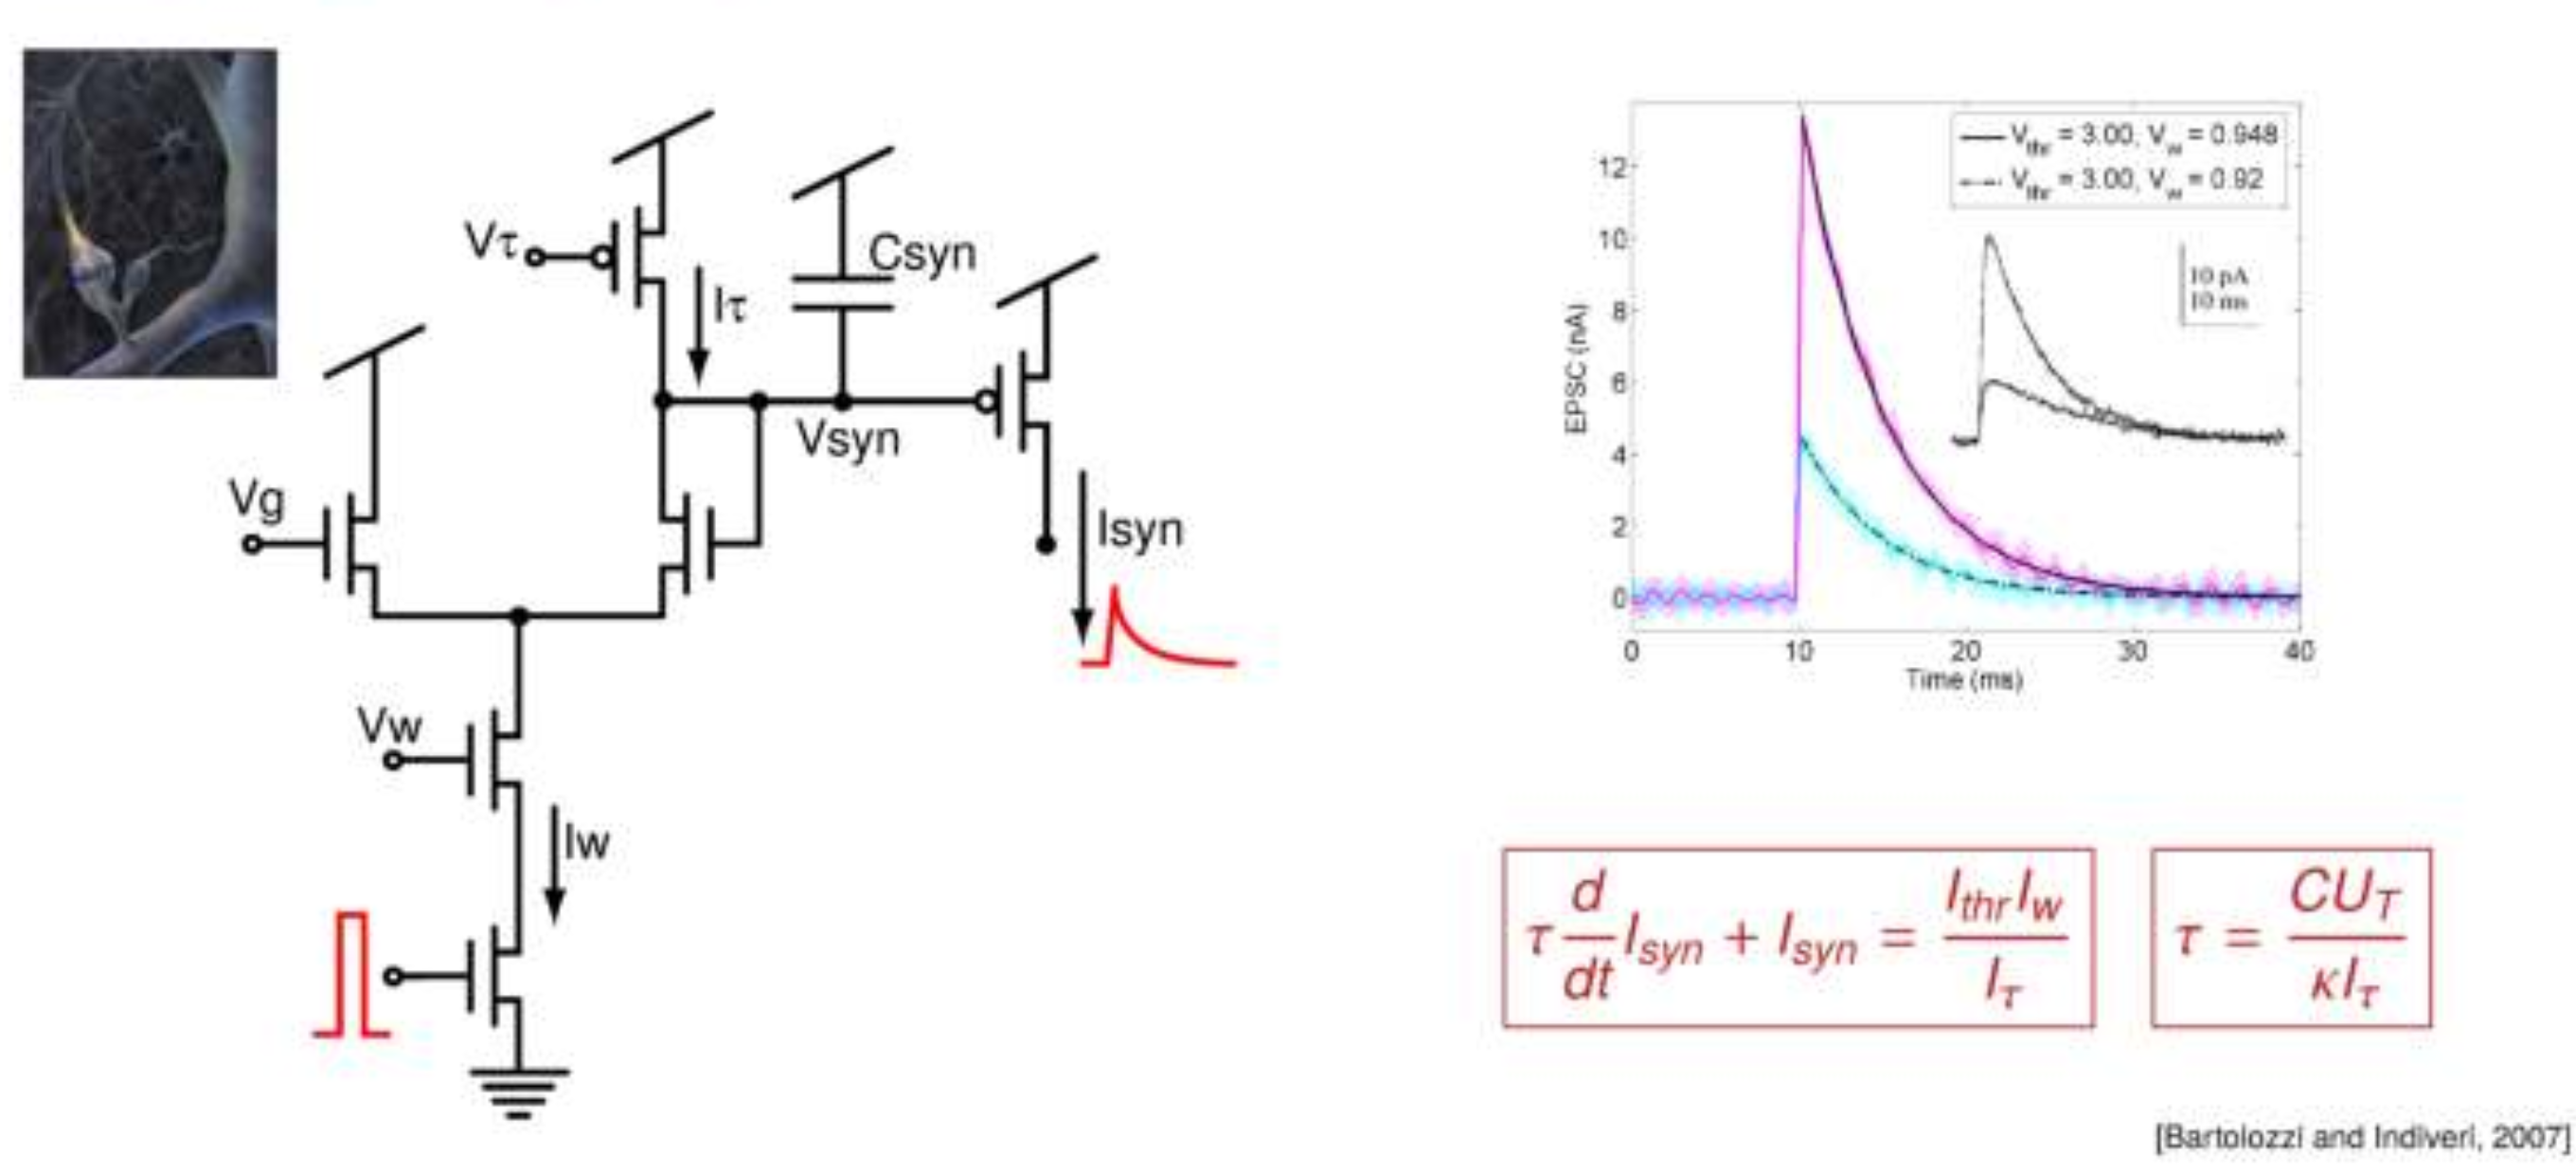
\includegraphics[width=0.8\linewidth]{12_NeuromorphicSystems2/figures/dpi.PNG}
    \caption{Differential Pair Integrator circuit.}
    \label{fig:dpi}
\end{figure}
%
Additional circuits can be attached to the DPI synapse to extend the model with extra features typical of biological synapses and implement various types of plasticity. For example, by adding two extra transistors, we can implement voltage-gated channels that model NMDA synapse behavior. Similarly, by using two more transistors, we can extend the synaptic model to be conductance based (Kandel, Schwartz, & Jessell, 2000). Furthermore, the DPI circuit is compatible with previously proposed circuits for implementing synaptic plasticity, on both short timescales with models of short-term depression (STD) (Rasche & Hahnloser, 2001; Boegerhausen, Suter, & Liu, 2003) and on longer timescales with spike-based learning mechanisms, such as spike timing-dependent plasticity (STDP).

The DPI neuron circuit is a variant of the generalized I&F neuron and is depicted in Figure \ref{fig:dpi-neuron}. The input DPI low-pass filter (yellow, ML1 - ML3) models the neuron’s leak conductance. A spike event generation amplifier (red, MA1 - MA6) implements current-based positive feedback (modeling both sodium activation and inactivation conductances) and produces address-events at extremely low-power. The reset block (blue, MR1 - MR6) resets the neuron and keeps it in a reset state for a refractory period, set by the $V_{ref}$ bias voltage. An additional DPI filter integrates the spikes and produces a slow after hyper-polarizing current $I_g$ responsible for spike-frequency adaptation (green, MG1 - MG6). 

%
\begin{figure}[h]
    \centering
    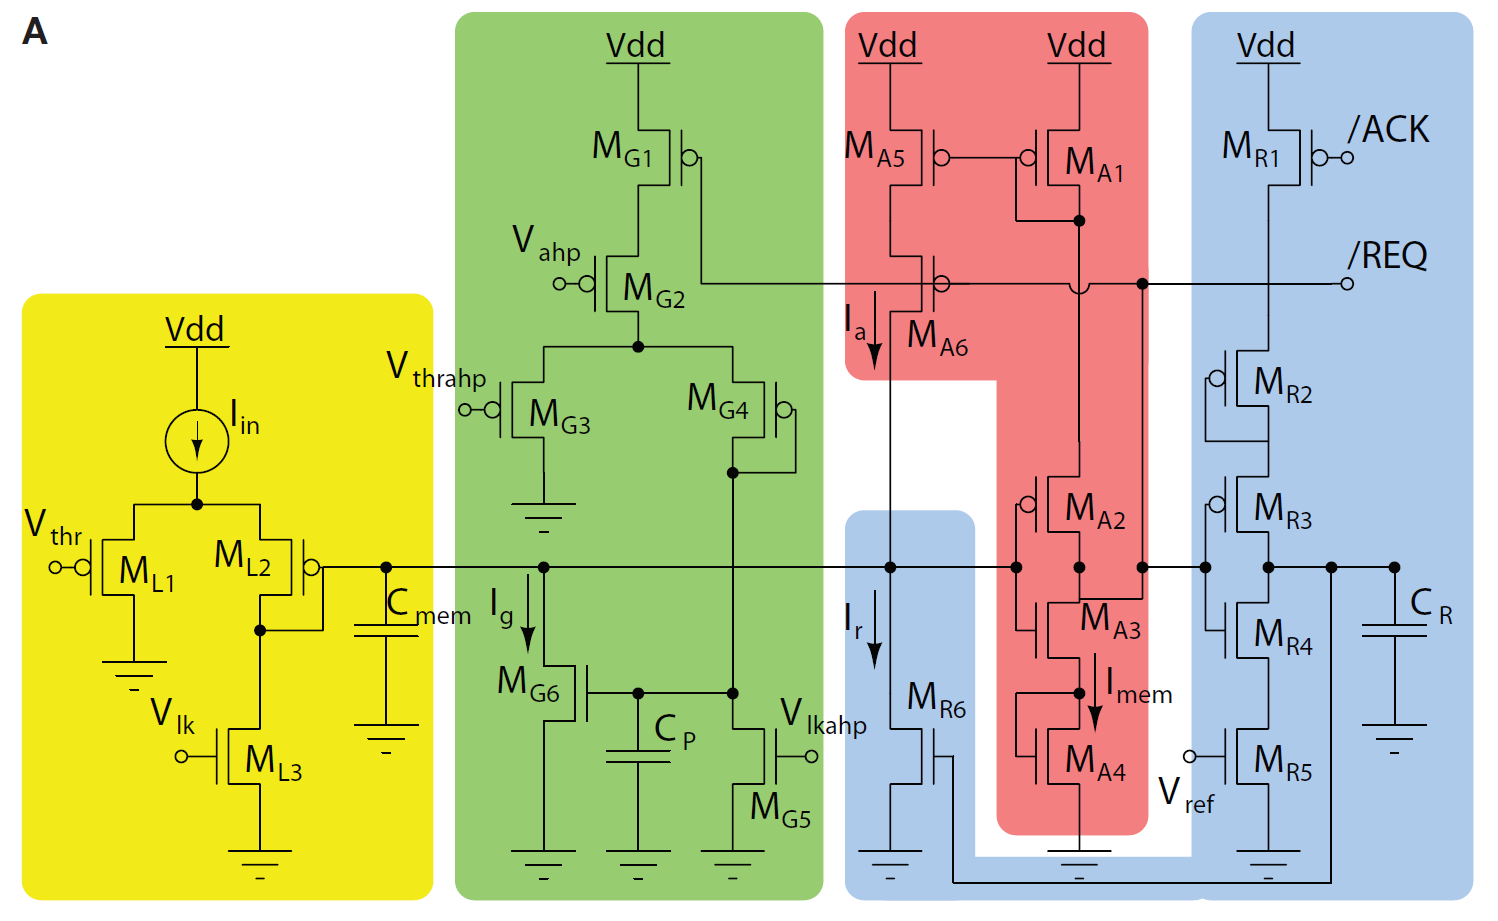
\includegraphics[width=0.8\linewidth]{12_NeuromorphicSystems2/figures/dpi_neuron.PNG}
    \caption{Differential Pair Integrator Neuron.}
    \label{fig:dpi-neuron}
\end{figure}
%

By applying a current-mode analysis to both the input and the spike-frequency adaptation DPI circuits, it is possible to derive a simplified analytical solution:

\begin{align}
    \tau \frac{d}{dt}I_{mem} + I_{mem} &\approx \frac{I_{th}I_{in}}{I_{\tau}} -I_g + f(I_{mem})\\
    \tau_{ahp}\frac{d}{dt}I_{g}+I_{g} &= \frac{I_{thrI_{ahp}}}{I_{\tau_{ahp}}}
\end{align}

The state of the art version of this neuron circuit consumes one order of magnitude less power than the circuit depicted in Figure \ref{fig:dpi-neuron} and two orders of magnitude less power than the digital implementation of the I\&F neuron. 

Given the exponential nature of the generalized I&F neuron’s non-linear term $f(I_{mem})$, the DPI-neuron implements an adaptive exponential I&F model (Brette and Gerstner, 2005). This I&F model has been shown to be able to reproduce a wide range of spiking behaviors, and explain a wide set of experimental measurements from pyramidal neurons. [silicon neuron circuits]

\subsubsection{Neuromorphic processors}

%
\begin{figure}[h]
    \centering
    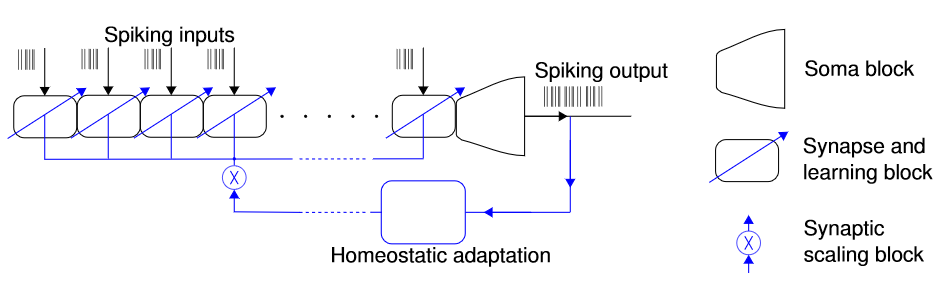
\includegraphics[width=0.8\linewidth]{12_NeuromorphicSystems2/figures/chips.PNG}
    \caption{}
    \label{fig:chip}
\end{figure}
%

Typical  spiking  neural  network chips have the elements described in Figure \ref{fig:chip}. Multiple instances of  these  elements  can  be  integrated  onto  single  chips  and connected  among  each  other  either  with  on-chip  hard-wired connections or via off-chip reconfigurable connectivity infrastructures. The most relevant characteristics of processors build based on analog circuits working in subthreshold are:

\begin{itemize}
    \item Slow temporal, non-linear dynamics
    \item Massively parallel operation
    \item Inhomogeneous, imprecise and noisy
    \item Adaptation and learning is done at multiple time-scales
    \item Fault tolerant and mismatch insensitive by design
    \item Fast asynchronous digital routing circuits
    \item Re-programmable network topology and connectivity
\end{itemize}

\subsection{Neuromorphic processing chips}

\subsubsection*{Neuromorphic agents}
When building processing chips, one can be inspired from life-forms that have brain and use them in every-day tasks, like mammals, insects etc. The physical properties of computational elements in brains can also be used as a reference from the computational resource usage standpoint, for example a bee's brain has a weight of 1 mg, a volume of 1 $mm^3$ and manages to squeeze almost 1 million neurons in it. The energy per operation is approximated to $10^{-15} J/spike$. Functional principles used by these life-forms can be used in the development of neuromorphic agents. Some of these are:

\begin{enumerate}
    \item Exploiting physical space in the most efficient way possible (e.g. squeezing cortical collumns in the neocortex)
    \item Let time represent itself
    \item Use both analog and digital computing elements
    \item Exploit non-linearities and temporal dynamics
    \item Leverage noise, variability and stochasticity
    \item Minimize wiring (maximize local connectivity)
    \item Optimize for processing complex spatio-temporal (dynamic and noisy) signals
    \item Re-use computational principles for sensory processing, motor control and cognitive computing
\end{enumerate}

\subsubsection*{DYNAP-SEL}
The DYNAP-SEL (Dynamic Neuromorphic Aynch Processor with Self Learning) is built based on an analog and digital co-design. It has on-chip inference and learning but also provides a reconfigurable architecture. The SRAM and TCAM memory cells are distributed and it uses capacitors for state dynamics. It is considered to be ideal for integration with binary, non-volatile resistive memory devices, for integration with dynamic, volatile/non-volatile memristive devices and can be integrated in 3D VLSI technology. It has a batter Fan In/Out and can do 12x more synaptic operations per second per watt than True North. It also uses 5x less energy per synaptic event and more than 2x less energy per spike.

\subsubsection*{Neuromorphic vs. conventional processors}
\begin{table}[h]
\begin{tabular}{|c|c|}
\hline
\textbf{Pros}       & \textbf{Cons} \\ \hline
Low-latency         & Limited resolution \\ \hline
Ultra low-power     & High variability, noisy \\ \hline
\end{tabular}
\end{table}

\begin{table}[h]
\begin{tabular}{|c|c|}
\hline
\textbf{Good}  & \textbf{Bad} \\ \hline
Real-time sensory-motor processing & High accuracy pattern recognition\\ \hline
Sensory fusion and on-line classification & High precision number crunching \\ \hline
Low-latency decision making & Batch processing of data sets \\ \hline
\end{tabular}
\end{table}

Programming a neuromorphic chip involves:

\begin{enumerate}
    \item defining the neural computational primitives
    \item composing multiple primitives for context dependent processing
    \item configuring the network structure and parameters
    \item training the neural network with different learning methods
\end{enumerate}

\subsubsection{Configuring}

\subsubsection*{Robot navigation}
In this work, a mixed-signal analog-digital neuromorphic processor ROLLS was interfaced with a neuromorphic dynamic vision sensor (DVS) mounted on a robotic vehicle. An autonomous neuromorphic agent that is able to perform neurally inspired obstacle-avoidance and target acquisition was developed. The implemented neuronal architectures for obstacle avoidance, presented in Figure \ref{fig:robo}: Violet OL and OR circles represent obstacle detecting neuronal populations. Orange DL and DR circles are motor driving populations. sp is the speed-setting population, and exp is the constantly firing population that sets the default speed. Thin arrows show excitatory non-plastic connections realized on the ROLLS chip, whereas colors and numbers show the weights.

%
\begin{figure}[h]
    \centering
    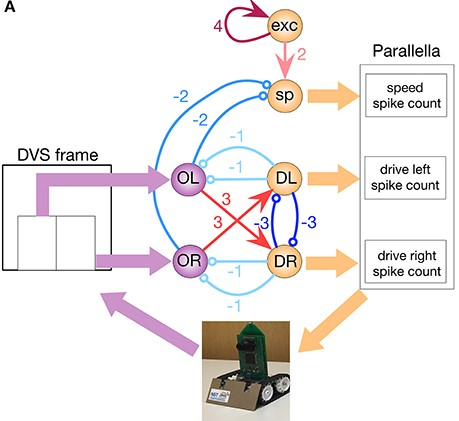
\includegraphics[width=0.8\linewidth]{12_NeuromorphicSystems2/figures/robo.jpg}
    \caption{Robotic navigation using neuromorphic processors.}
    \label{fig:robo}
\end{figure}
%

\subsubsection*{On-line detection of iEEG High-Frequency Oscillations (HFO)}

An HFO is a series of spontaneous EEF events in the frequency range between 80 and 500 Hz consisting of at least four oscillations that clearly stand out from the baseline. HFO in human iEEG are used to identify epileptogenic brain tissue during epilepsy surgery. However, current methods typically analyse the raw data offline using complex time-consuming algorithms so NCS group at INI developed a compact neuromorphic sensory processing system-on-chip that can monitor the iEEG signals and detect high frequency oscillations in real-time using spiking neural networks.

The integrated device has an analog front-end that can extract predefined spectral features and encode them as address-events, and a neuromorphic processor core that implements a network of integrate and fire neurons with dynamic synapses. The front-end amplifies the bio-signals, filters them in specific frequency bands and converts filter outputs to asynchronous events. The DYNAP block is configured to implement a spiking neural network which receives these events, processes them via its dynamic synapses and neurons, and detects HFO in two different frequency bands.

The Low Noise Amplifier is the most critical block employed in the front-end, which ensures linear amplification and systematic noise suppression. It includes an Operational Transconductance Amplifier (OTA) in capacitive feedback configuration with MOS Bipolar structure as resistive elements.

%
\begin{figure}[h]
    \centering
    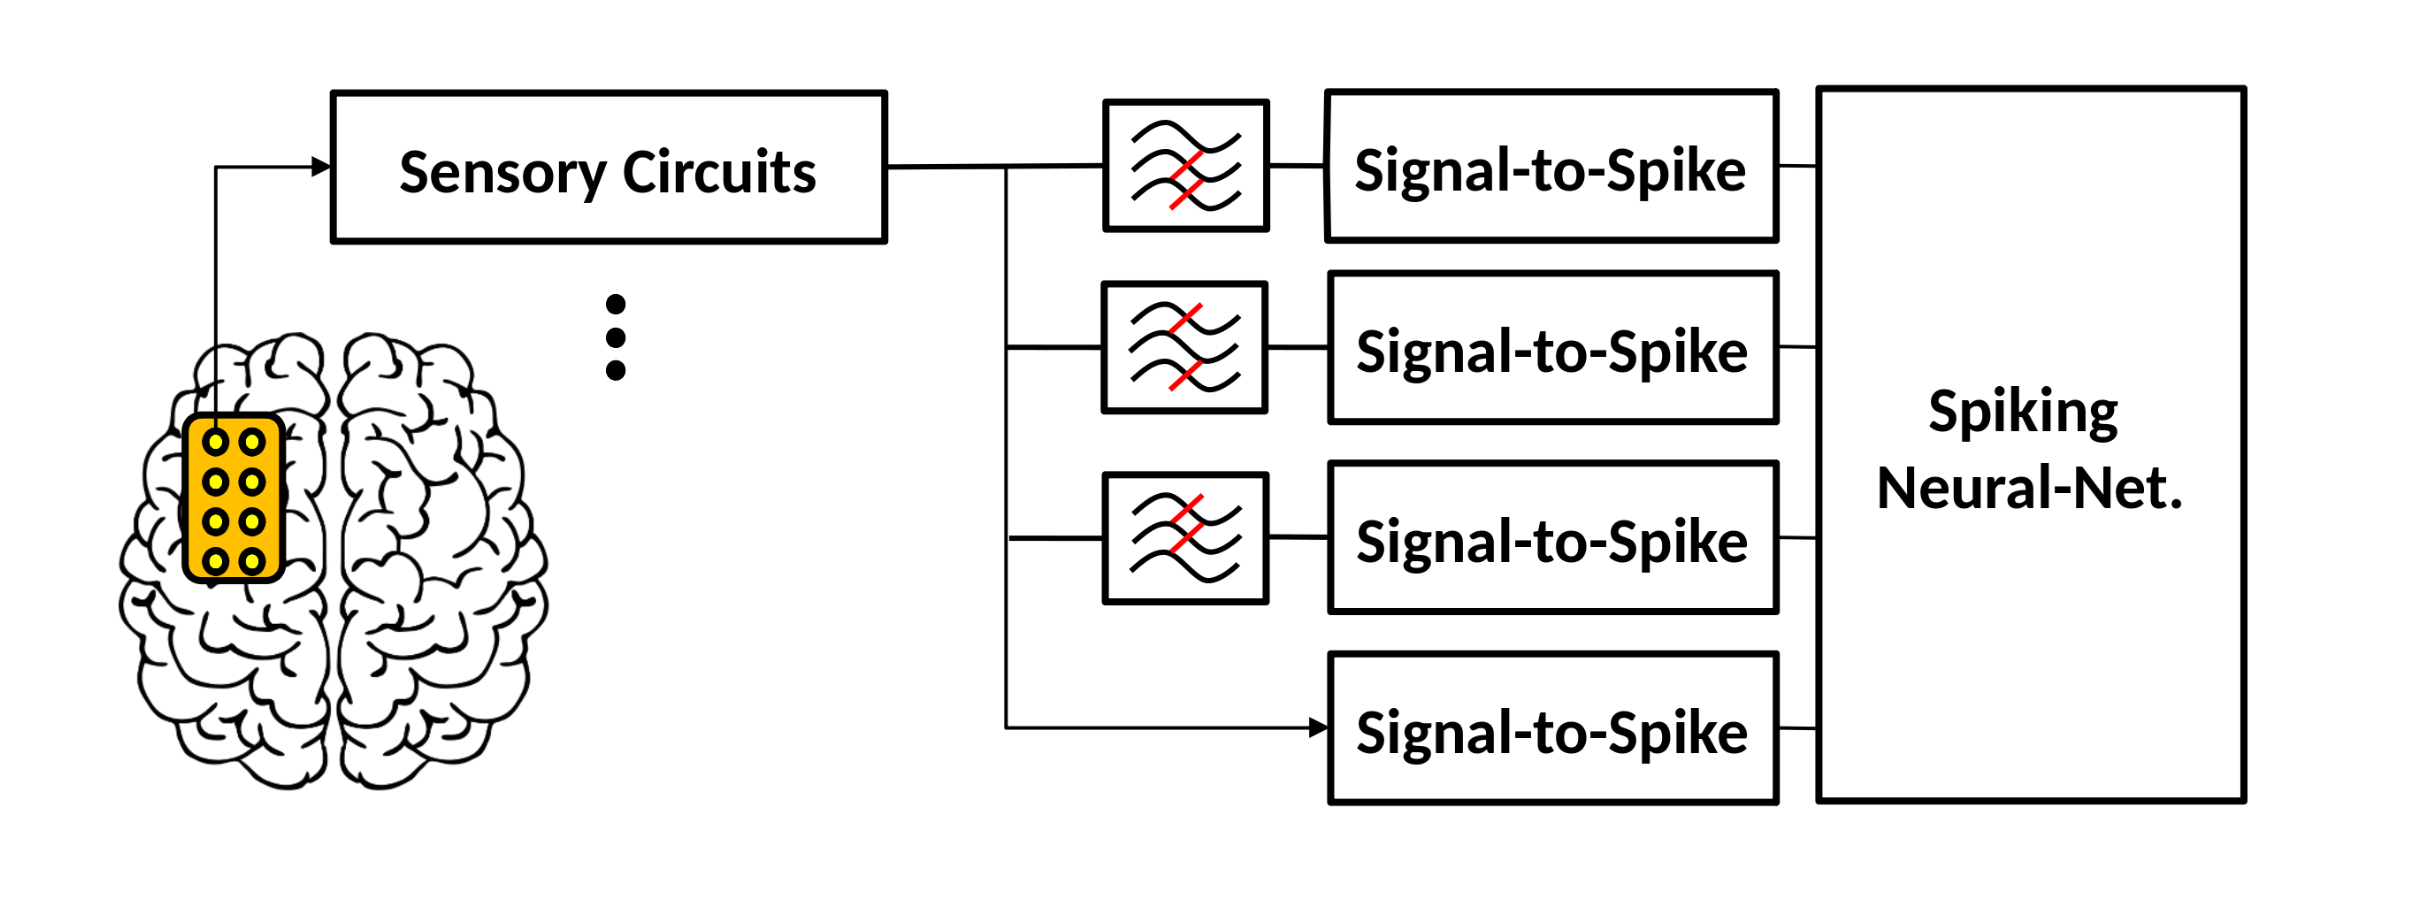
\includegraphics[width=0.8\linewidth]{12_NeuromorphicSystems2/figures/eeg.PNG}
    \caption{On-line detection of iEEG HFO.}
    \label{fig:eeg}
\end{figure}
%

Another important component of the analog front-end is the asynchronous ADC, which enables the analog front-end to interface with the event-based processing core and translates the input data to a sequence of spikes. Here, each spike corresponds to a polarized, adjustable amount of change
in the analog input signal.

The estimated power consumption of the front-end is $6.2 \micro W$/channel and the area-on-chip for a single channel is 0.15 square millimetres. The SNN classifier provides 90.5\% sensitivity and 67.7\% specificity for detecting high frequency oscillations. This is the first feasibility study towards identifying relevant features in intracranial human data in real-time on-chip using event-base processors. [cite from lecture]

\subsubsection{On-line classification of EMG signals}

An accurate description of muscular activity plays an important role in the clinical diagnosis and rehabilitation research. The electromyography (EMG) is the most used technique to make accurate descriptions of muscular activity. The EMG is associated with the electrical changes generated by the activity of the motor neurons. Typically, to decode the muscular activation during different movements, a large number of individual motor neurons are monitored simultaneously, producing large amounts of data to be transferred and processed by the computing devices. In this paper, an alternative approach is followed, that can be deployed locally on the sensor side. It proposed a neuromorphic implementation of a spiking neural network (SNN) to extract spatio-temporal information of EMG signals locally and classify hand gestures with very low-power consumption. A mixed-signal analog/digital neuromorphic processor was used

%
\begin{figure}[h]
    \centering
    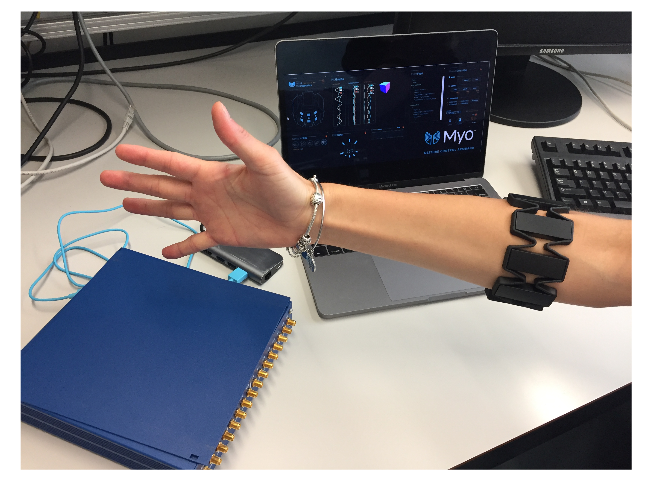
\includegraphics[width=0.8\linewidth]{12_NeuromorphicSystems2/figures/myo.PNG}
    \caption{MYO device used obtain EMG signals}
    \label{fig:myo}
\end{figure}
%

%
\begin{figure}[h]
    \centering
    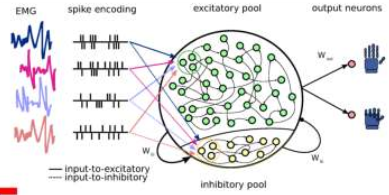
\includegraphics[width=0.8\linewidth]{12_NeuromorphicSystems2/figures/stages.PNG}
    \caption{Processing pipeline of input EMG data, encoded in AER, passing through the reservoir and ending into the actuators.}
    \label{fig:stage}
\end{figure}
%

EMG signals related to two movements of open and closed hand gestures were recorded, then converted into asynchronous Address-Event Representation (AER) signals. These signals were provided as input to a recurrent spiking neural network implemented on an ultra-low power neuromorphic chip and the chip’s  response was analyzed. The  recurrent network was configured as a Liquid State Machine (LSM) as a means to classify the spatio-temporal data. The Separation Property (SP) of the liquid  states was evaluated for the  two  movements. Results show that the activity of the silicon neurons can be encoded in state variables for which the average state distance is larger between two different gestures than it is between the same ones measured across different trials.

The LSM type of RNNs proposes the ingenious idea of a two layer network comprised of spiking neurons with dynamic synapses in which the first layer is set up with randomly connected recurrent weights to project the input signal to a higher dimensional space. The complex dynamics of the synapses and neurons, and the high dimensional space provide a pool of basis functions on which the projected data can be separated because of the Kernel properties of the LSM. As a result, the second layer can simply be trained on the basis of a gradient decent learning rule which is powered by the already separated data from the first random layer. The synapse and neural dynamics are directly and faithfully emulated by the analog circuits of neuromorphic chips and the high variability of the LSM, imposed in software by the randomness of the first layer weights is easily achieved on the neuromorphic chips when using sub-threshold analog circuits to implement the neuron and synapse circuits. [cite from lecture]

\subsubsection{Learning}

There exist many pre-synaptic (input) driven learning algorithms that are hardware friendly, but all have in common 3 main aspects:

\begin{itemize}
    \item Bi-stable synapses
    \item Redudancy
    \item Variability
\end{itemize}

\subsubsection*{Ensemble learning}

Intrinsic variability  and  diverse  activation  patterns  are  often  identified as fundamental aspects of neural computation for information maximization and transmission. The strategy of combining large numbers of variable and imprecise computing elements to carry out robust computation is also followed by a wide set of traditional machine learning approaches. These approaches work on the principle of combining the output of multiple inaccurate computational modules that have slightly different properties, to optimize classification performances and achieve or even beat the performances of single accurate and complex learning systems. A set of similar theoretical studies showed that the coexistence of multiple different time-scales of synaptic plasticity (e.g., present due to mismatch in the time-constants of the DPI synapse circuits) can dramatically improve the memory performance of ANN. [chica et al]

\subsubsection*{Hopfield/attractor networks} \label{wta}

Mechanisms operating at the network level can also allow neural processing systems to form short-term memories, consolidate long-term ones, and carry out nonlinear processing functions such as selective amplification (e.g.,to implement attention and decision making). An example of such a network-level mechanism is provided by "attractor networks." These are networks of neurons that are recurrently connected via excitatory synapses, and that can settle into stable patterns of firing even after the external stimulus is removed. Different stimuli can elicit different stable patterns, which consist of specific subsets of neurons firing at high rates. Each of the high-firing rate attractor states can represent a different memory. To make an analogy with conventional logic structures, a small attractor network with two stable states would be equivalent to a flip-flop gate in CMOS. 

%
\begin{figure}[h]
    \centering
    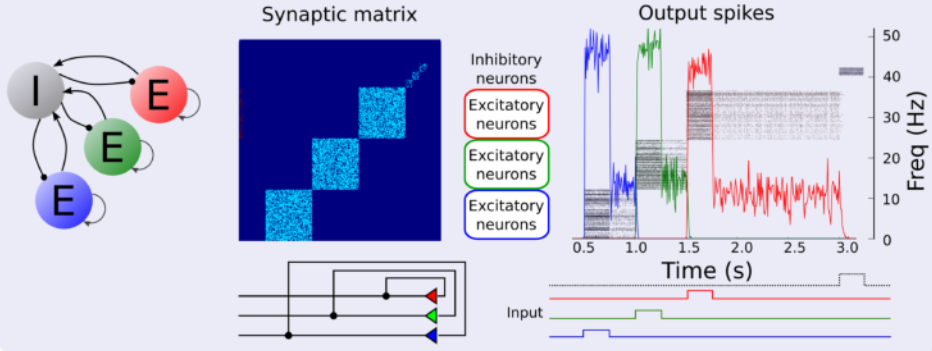
\includegraphics[width=0.8\linewidth]{12_NeuromorphicSystems2/figures/wta.PNG}
    \caption{Hopfield - attractor - winner-takes-all networks}
    \label{fig:wta}
\end{figure}
%

A particularly interesting class of attractor networks is the one of soft winner-take-all (sWTA) neural networks. In these networks, groups of neurons both cooperate and compete with each other. Cooperation takes place between groups of neurons spatially close to each other, while competition is typically achieved through global recurrent patterns of inhibitory connections. When stimulated by external inputs, the neurons excite their neighbors and the ones with highest response suppress all other neurons to win the competition. Thanks to these competition and cooperation mechanisms, the outputs of individual neurons depend on the activity of the whole network and not just on their individual inputs. [indiveri,liu 205]

\subsubsection*{Spike-based back-propagation}
Discussed in Zenke's lecture.

\subsubsection*{Long eligibility traces}
To achieve long biological realistic time-scales that do not interfere with signal transmission and learning, it is necessary to develop circuits with time scales that range from seconds to hours. In order to optimize the circuit’s area to allow the dense integration of thousands of synapses and neurons on a single chip, the capacitance of the homeostatic control circuits must be small, therefore long time scales can only be achieved by extremely small currents. An example of such a circuit is the ultra-low leakage cell shown in Figure \ref{fig:cell}. This circuit increases or decreases its output voltage $V_{thr}$ by controlling the direction of a very small current across the channel of the LLC p-FET to slowly charge or discharge the capacitor $C_F$. 

%
\begin{figure}[h]
    \centering
    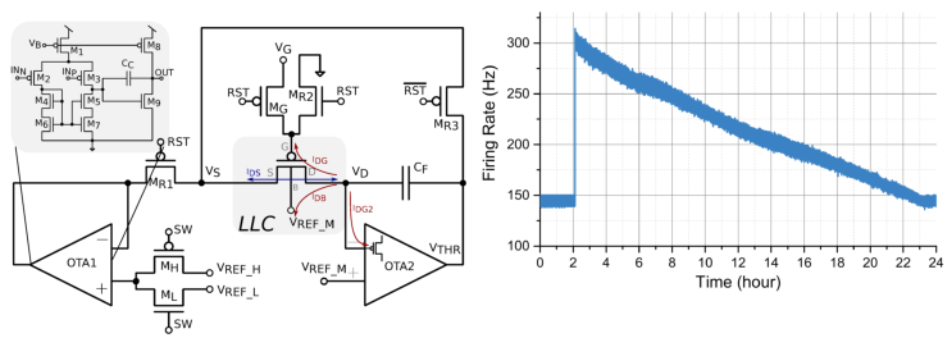
\includegraphics[width=0.8\linewidth]{12_NeuromorphicSystems2/figures/cell.PNG}
    \caption{Low Leakage Cell and its long eligibility trace}
    \label{fig:cell}
\end{figure}
%

\subsubsection*{Three factor learning circuits}

Event-driven neuromorphic hardware with on-line learning capabilities enables the low-power local processing of signals on the edge sensors. Implementing such hardware requires having an always-on online learning operation in order to continuously adapt to the changes in the environment. Therefore, as the data is continuously streaming, there cannot be a separation between the training and the testing phase. Such constraint thus asks for a continuous time learning strategy which includes a mechanism to stop changing the weights when the system has reached an optimal operating point, so that it does not over-fit the input data and it generalizes to unseen patterns of the learned class. Circuits with spike-based local gradient-descent learning rule are proposed, that comprise also this additional “stop-learning” feature and that have a wide range of configurability options over the learning parameters. 

In this paper, the authors propose spike-based circuits implementing a local  gradient-descent  based  learning  rule  (delta  rule)  which is empowered by the additional stop-learning feature. This is done through a modified version of the Bump circuit.

The learning circuits implement Delta-rule which is a learning algorithm minimizing the Least Mean Square (LMS) error of a single-layer neural network whose cost function is defined as the difference between a target desired output signal T and the network output signal y, for a given set of input patterns signals x, weighted by the synaptic weight parameters w. Specifically, this learning rule, given the learning rate $\alpha$, sets the corresponding weight change between the $i^{th}$ input and the $j^{th}$ output neuron to be:

\begin{equation}
    \delta w = \alpha (T_j-y_j)x_i
\end{equation}

This algorithm was previously implemented using the Bump circuit by comparing the rate of the neuron spikes to a target value. The rates are calculated through low-pass filtering the spikes by using a Diff-Pair Integrator (DPI) circuit which receives spike inputs, low pass filters them, and generates output currents proportional to the rate of the spikes. The Bump circuit provides us with the analog value and the direction of the difference between the neuron’s and target’s spike rate, along with a flag for the similarity between the two signals which is ideal for implementing Delta update rule. 


The width of the transfer characteristics of the Bump current is a dead region where the target and the neuron are ”similar enough”. This dead region directly implements the ”stop-learning” region where the error of the network is close to negligible and hence no update in the synaptic weights is necessary. The VW Bump circuit has the advantage of having an electrical control over the width of the bump current characteristic function.

%
\begin{figure}
     \centering
     \begin{subfigure}[b]{0.47\textwidth}
        \centering
        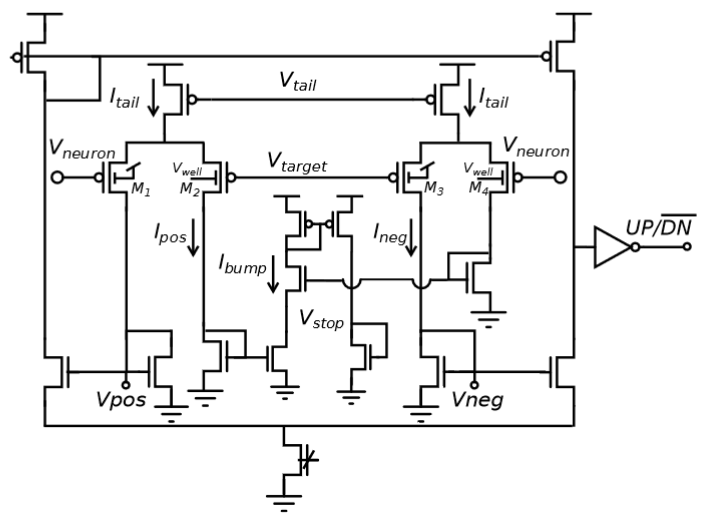
\includegraphics[width=\textwidth]{12_NeuromorphicSystems2/figures/vwbump.PNG}
        \caption{}
        \label{fig:v_max}
     \end{subfigure}
     \hfill
     \begin{subfigure}[b]{0.47\textwidth}
         \centering
        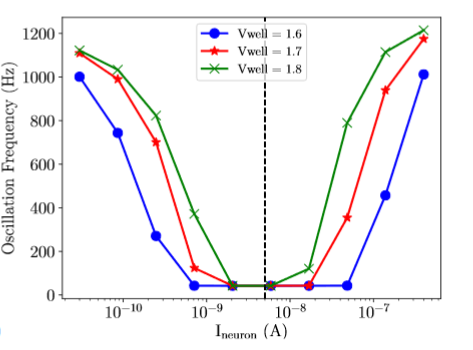
\includegraphics[width=\textwidth]{12_NeuromorphicSystems2/figures/dead.PNG}
        \caption{}
        \label{fig:ex2_epsc_max}
     \end{subfigure}
        \caption{VWBump circuit and the stop-learning region controlled by the back-gate voltage $V_w$}
        \label{fig:ex2_1}
\end{figure}
%

\subsection{Computational primitives}
\subsubsection{Cortical microcircuit}

The cortical microcircuit explains the intracellular responses to pulse stimulation in terms of the interactions between three basic populations of neurons, and reveals the following features of cortical processing that are important to computational theories of neocortex. First, inhibition and excitation are not separable events. Activation of the cortex inevitably sets in motion a sequence of excitation and inhibition in every neuron. Second, the thalamic input does not provide the major excitation arriving at any neuron. Instead the intracortical excitatory connections provide most of the excitation. Third, the time evolution of excitation and inhibition is far longer than the synaptic delays of the circuits involved. This means that cortical processing cannot rely on precise timing between individual synaptic inputs.

%
\begin{figure}[h]
    \centering
    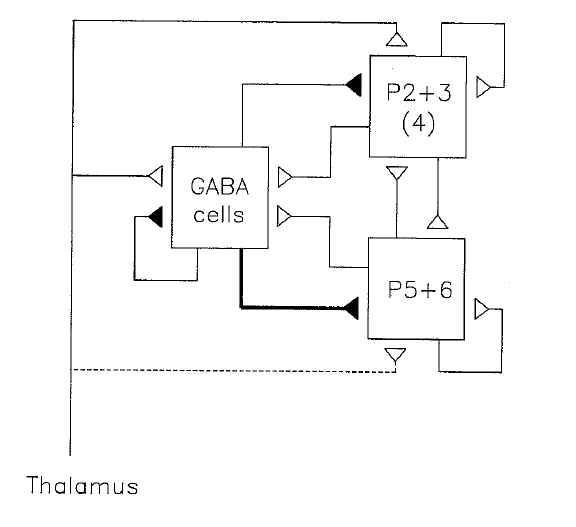
\includegraphics[width=0.8\linewidth]{12_NeuromorphicSystems2/figures/micro.PNG}
    \caption{Model of cerebral cortex that successfully predicts the intracellular
responses of cortical neurons to stimulation of thalamic afferents}
    \label{fig:micro}
\end{figure}
%

Three populations of neurons interact with one another: one population is inhibitory (GABA cells, solid synapses), and two are excitatory (open synapses), representing superficial (P2 + 3) and deep (P5 + 6) layer pyramidal neurons. The layer 4 spiny stellate cells are incorporated with the superficial group of pyramids. Each population receives excitatory input from the thalamus, which is weaker (dashed line) to deep pyramids. The inhibitory inputs activate both $GABA_A$ and $GABA_B$ receptors on pyramidal cells. The thick line connecting GABA tO P5+6 indicates that the inhibitory input to the deep pyramidal population is relatively greater than that to the superficial population. However, the increased inhibition is due to enhanced $GABA_A$ drive only. The $GABA_B$ inputs to p5+6 is similar to that applied to P2 + 3.

\subsubsection{WTA}
Discussed in section \ref{wta}.
\subsubsection{Intrinsic oscillators and Central Pattern Generators}
In animals, a basic block of locomotor control is the Central Pattern Generator (CPG), a neural network capable of generating coordinated pattern of rhythmic activity, driven by very simple input signals, which are sufficient to modulate locomotion patterns.  

In particular the animal that has been mostly studied in this context is the lamprey. In the lamprey the presence of mutually inhibitory connections organizes neurons in antagonist segments or units. The spinal cord system consists of about 100 units (segments), each containing an oscillatory neural network. In each of these segments the left-right alternated spiking activity has a frequency ranging from about 0.1 Hz to 8-10 Hz. Each side of a segment can generate bursting activity, independent of the other side. 

The setup used to implement the neural model comprises a mixed signal analog/digital VLSI device interfaced, for prototyping purposes, to a commercially available FPGA board. To provide the model’s input signal, we first created an oscillatory network on the chip. This network is composed of two pools of 4 silicon neurons that are sparsely and recurrently connected. Connectivity within each pool has ratio $c_{rec}=0.5$ (indicates the probability that a neuron in the pool connects to any other neuron in the same pool). The two pools inhibit each other via inhibitory connections with a connectivity ratio $c=0.5$. This interplay of recurrent excitation, spike-frequency adaptation and external inhibition creates a stable pattern of oscillation, when neurons are driven by a constant injection current.   

%
\begin{figure}
     \centering
     \begin{subfigure}[b]{0.47\textwidth}
        \centering
        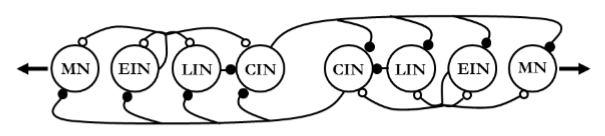
\includegraphics[width=\textwidth]{12_NeuromorphicSystems2/figures/cpg0.PNG}
        \caption{}
        \label{fig:cpg0}
     \end{subfigure}
     \hfill
     \begin{subfigure}[b]{0.47\textwidth}
         \centering
        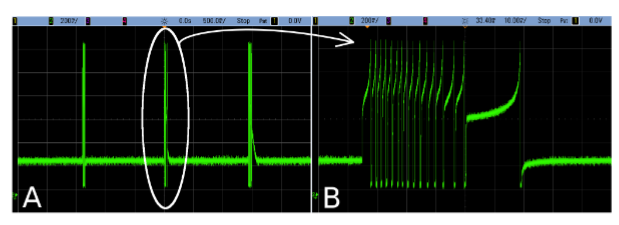
\includegraphics[width=\textwidth]{12_NeuromorphicSystems2/figures/cpg.PNG}
        \caption{}
        \label{fig:cpg1}
     \end{subfigure}
        \caption{A. Spinal cord  CPG unit, comprising two sides with multiple types of neurons. The neurons are coupled by both excitatory and inhibitory connections. Filled circles represent inhibitory synapses while open circles the excitatory. B. Silicon neuron measurements}
        \label{fig:cpg}
\end{figure}
%

The neuron produces periodic bursting, lasting approximately 60 ms. with an inter-burst interval of about 1.5 s. The spiking frequency during the burst is about 35 Hz.

\subsubsection{Perceptual bistability}
The ability of embodying information in the dynamics of a recurrent neural network, which can persist also in the absence of external stimulation and transition between meta-stable states, represents a fundamental processing capability of neural systems. In biologically-inspired neural network models, it has often been assumed that an attractor in phase space represents an internal or an external source of information. From a biological perspective, recurrent spiking neural network models have expressed the dynamics of bistability in their firing rates. The architecture of the network is illustrated in Figure \ref{fig:bista} is organized in three populations of neurons A, B and background (bg). The number of neurons in population A and B is $Na=Nb=22$, while the background population counts $Nbg=12$ neurons. Each population is recurrently connected, with sparse connectivity. Populations A and B inhibit each other via direct inhibitory connections. 

Long-lasting spiking activity in the cortex, that lasts much longer than the typical time scales of synapses and membrane potentials, is the neural correlate of working memory and perceptual decision making. In theoretical neuroscience models this activity is assumed to encode sensory inputs which relate to different alternative possible decisions or percepts. This activity is accumulated in different pools of neurons that, due to their recurrent excitatory connections, are capable of sustaining persistent activity, even after the input stimulus that triggered it is removed.

%
\begin{figure}
     \centering
     \begin{subfigure}[b]{0.47\textwidth}
        \centering
        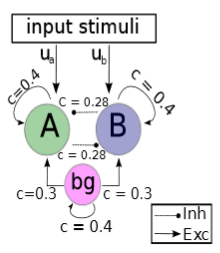
\includegraphics[width=\textwidth]{12_NeuromorphicSystems2/figures/bista.PNG}
        \caption{}
        \label{fig:cpg0}
     \end{subfigure}
     \hfill
     \begin{subfigure}[b]{0.47\textwidth}
         \centering
        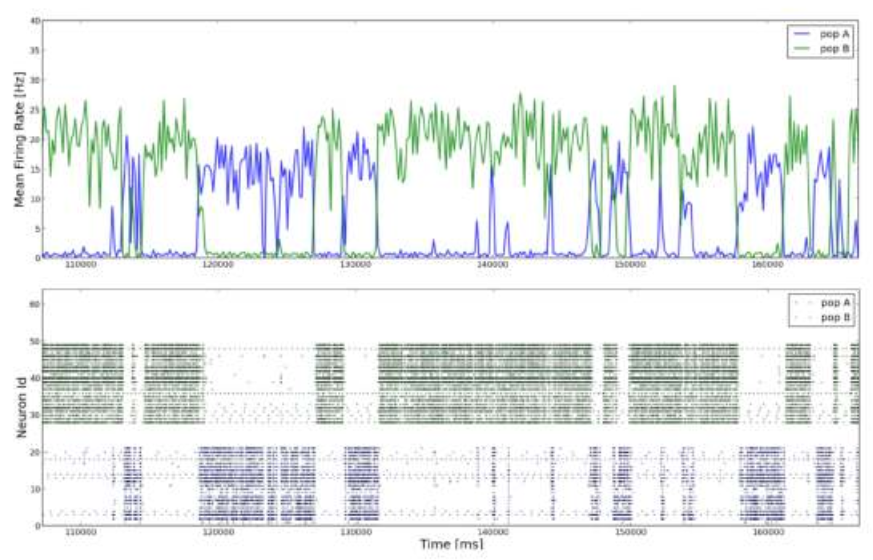
\includegraphics[width=\textwidth]{12_NeuromorphicSystems2/figures/bista2.PNG}
        \caption{}
        \label{fig:cpg1}
     \end{subfigure}
        \caption{A. Network structure B. Neuromorphic chip measurements}
        \label{fig:bista}
\end{figure}
%

The observed behaviour of the neuromorphic attractor network, when all neurons are stimulated by a constant injection of current, is an alternation of perceptual dominance among the two different activity states with very long time constants,  orders of seconds.  Figure \ref{fig:bista} shows five seconds of recordings of such behaviour. It shows the mean firing rate activity over time of neurons grouped in populations. Continuous green line depicts neurons in population A, and the dashed blue line represents neurons in population B. An irregular alternation of high activity is evident, and only one of the two populations of neurons can be found in the up state (∼80 Hz) of activity: this is a confirmation that the network is operating in a winner-take-all regime.
\subsubsection{Neural state machines}

A finite-state machine (FSM) is a mathematical model of computation used to design both computer programs and sequential logic circuits. It is conceived as an abstract machine that can be one of a finite number of states. State-dependent computation is one of the main signatures of cognition. Recently, it has been shown how it can be used as a computational primitive in spiking neural networks for constructing complex cognitive behaviors in neuromorphic agents. In spiking neural networks, Neural  State Machines (NSMs) provide a generic computational model for implementing state-dependent computations. Similar to finite-state automata, NSMs are defined by four sets of Boolean variables, which include a set of states $S={s1,s2,s3...}$, a set of excitatory input signals $E={e1,e2,e3...}$, a set of inhibitory input signals $I={i1,i2,i3...}$, and a set of transition signals $T={t1,t2,t3...}$. Each  transition  of T links one source state of S to at least one target state of S and is also linked to an additional set of input signals. The co-occurrence of input signals and source state signals are used to switch transitions on and off. 

%
\begin{figure}[h]
    \centering
    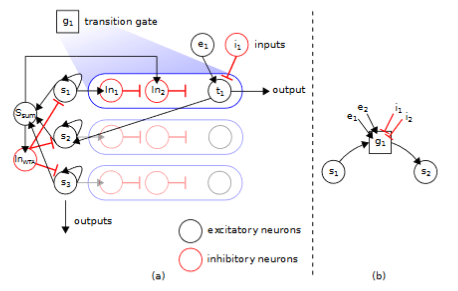
\includegraphics[width=0.8\linewidth]{12_NeuromorphicSystems2/figures/nsm0.PNG}
    \caption{NSM structure its schematic representation}
    \label{fig:nsm}
\end{figure}
%

Multiple NSMs can interact with each other. They have been used as a modular building block in Spiking Neural Networks (SNNs) to construct complex cognitive computations in neuromorphic agents, such as solving Constraint Satisfaction Problems (CSPs). Synthesis of a target FSM in neuromorphic VLSI neural networks is presented in Figure \ref{fig:nsm}.

%
\begin{figure}[h]
    \centering
    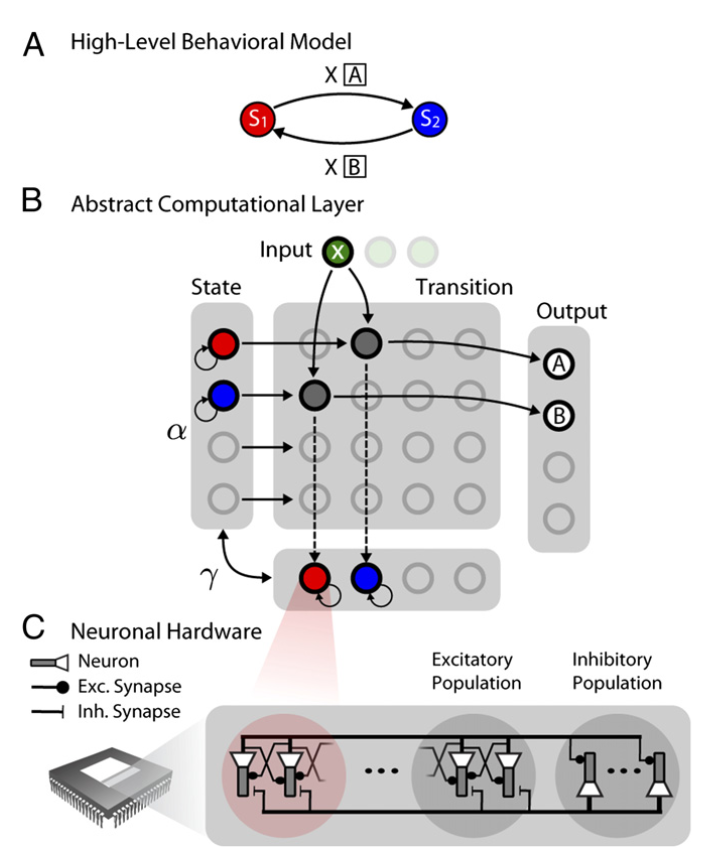
\includegraphics[width=0.8\linewidth]{12_NeuromorphicSystems2/figures/nsm.PNG}
    \caption{FSM synthesis}
    \label{fig:nsm}
\end{figure}
%

 Subfigure (A) contains the state diagram of the high-level behavioral model. Circles represent states and arrows indicate the transitions between them, conditional on input symbol X. In this example state machine, the active state flips between $S_1$ and $S_2$ in response to X and outputs either the response A or the response B, depending on the previous state. 
 
 Subfigure (B) represents the computational substrate composed of three sWTA networks: two “state-holding” networks (vertical and horizontal rectangles) and a third transition network (central square). The shaded circles in each sWTA represent populations of spiking neurons that are in competition through a population of inhibitory neurons (not displayed). The state-holding sWTA networks are coupled population-wise (γ-labeled arrow, red with red, blue with blue, etc.) to implement working memory. Solid arrows indicate stereotypic couplings, and the dashed arrows indicate couplings that are specific to the FSM (in this case the one shown in A). The gain and threshold in the transition sWTA are configured such that each population becomes active only if both of its inputs are presented together. The sWTA competition ensures that only a single population in the network is active at any time. An additional output sWTA network is connected to the transition network to represent the output symbols. To program a different state machine, only the dashed arrows need to be modified. 
 
 Subfigure (C) depicts the multineuron chips used in the neuromorphic setup, whicj feature a network of low-power I&F neurons with dynamic synapses. The chips are configured to provide the hardware neural substrate that supports the computational architecture consisting of sWTA shown in B. Each population of an sWTA network is represented in hardware by a small population of recurrently coupled spiking neurons ($N=16$), which compete against other populations via an inhibitory population. [neftci 2013]
\subsubsection{WTA-based constraint-satisfaction problems}

Mostafa et al. proposes a recurrent neural network modeled as a continuous-time dynamical system, that can solve constraint satisfaction problems. Discrete variables are represented by coupled Winner-Take-All (WTA) networks, and their values are encoded in localized patterns of oscillations that are learned by the recurrent weights in these networks.

The basic building block of the proposed network is the WTA circuit in which multiple excitatory populations are competing through a common inhibitory population. When the excitatory populations of the WTA network receive inputs of different amplitudes, their activity will increase and be amplified due to the recurrent excitatory connections. This will in turn activate the inhibitory population which will suppress activity in the excitatory populations until an equilibrium is reached. Typically, the excitatory population that receives the strongest external input is the only one that remains active (the network has selected a winner). By properly tuning the connection strengths, it is possible to configure the network so that it settles into a stable state of activity (or an attractor) that persists after input removal.

Constraints over the variables are encoded in the network connectivity. Although there are no sources of noise, the network can escape from local optima in its search for solutions that satisfy all constraints by modifying the effective network connectivity through oscillations. If there is no solution that satisfies all constraints, the network state changes in a seemingly random manner and its trajectory approximates a sampling procedure that selects a variable assignment with a probability that increases with the fraction of constraints satisfied by this assignment. External evidence, or input to the network, can force variables to specific values. When new inputs are applied, the network re-evaluates the entire
set of variables in its search for states that satisfy the maximum number of constraints, while being consistent with the external input.

The results demonstrate that the proposed network architecture can perform a deterministic search for the optimal solution to problems with non-convex cost functions. The network is inspired by canonical microcircuit models of the cortex and suggests possible dynamical mechanisms to solve constraint satisfaction problems that can be present in biological networks, or implemented in neuromorphic electronic circuits.

\subsection{Conclusion}

The main research objective is to implement computational neuroscience models in low-power, mixed signal, hybrid memristive/CMOS technology to build efficient on-line learning and processing systems.

An important guiding principle is exploiting the physics of semiconductors to implement efficient neuromorphic cognitive agents that interact intelligently with the environment.
\end{document}